\chapter{Новые результаты}


\begin{enumerate}
    \item ординарный каскад с прямым обогащением регенерата (не выполняется огр-е на $C^{232}_{\text{P}}$ и отсутствует компенсация $^{236}$U)
    \item каскад с разбавлением регенерата на входе
    \item каскад с разбавлением регенератом предварительно обогащенного природного урана;
    \item каскад с двумя потоками питания (R-каскад) без компенсации $^{236}$U
    \item двойной каскад с компенсацией $^{236}$U
    \item Двойной модифицированный аскад
\end{enumerate}


\begin{table}
    \begin{tabular}{c|cccccc}
        $\text{П-р | Схема}$ & $\text{1}$ & $\text{2}$ & $\text{3}$ & $\text{4}$ & $\text{5}$ & $\text{6}$\\ \hline
        $\text{$Y_{f}$}$ & $0.95$ & $5.5e-6$ & $0.87$ & $1.0$ & $0.65$ & $0.87$\\ \hline
        $\text{$Y_{E}$}$ & $0.95$ & $2.1$ & $1.0$ & $5.1$ & $0.65$ & $0.84$\\ \hline
        $\text{$\delta(\frac{\Delta A}{P}), \%$}$ & $5.9$ & $4.1$ & $12.0$ & $11.0$ & $23.0$ & $11.0$\\ \hline
        $\text{$\delta(\frac{F_{NU}}{P}), \%$}$ & $100.0$ & $710.0$ & $0.21$ & $21.0$ & $100.0$ & $19.0$\\ \hline
        $\frac{P_{2}}{P}$ & $0$ & $0$ & $0$ & $0$ & $0$ & $0.011$\\ \hline
        $\text{$C^{232}_{\text{P}}, \%$}$ & $2.4e-6$ & $5.0e-7$ & $6.6e-9$ & $5.0e-7$ & $5.0e-7$ & $4.9e-7$\\ \hline
        $\text{$C^{234}_{\text{P}}, \%$}$ & $0.12$ & $0.065$ & $0.042$ & $0.057$ & $0.19$ & $0.06$\\ \hline
        $\text{$C^{235}_{\text{P}}, \%$}$ & $4.95$ & $5.0$ & $4.95$ & $4.95$ & $7.72$ & $5.1$\\ \hline
        $\text{$C^{236}_{\text{P}}, \%$}$ & $2.9$ & $0.19$ & $0.0099$ & $0.61$ & $9.5$ & $0.66$
        \end{tabular}        
\caption{Сравнение интегральных показателей схем.{\label{55555}}}
\end{table}

% Попробовал посчитать с перебором $M_{k1}$ и $M_{k2}$, так как для  всех 4 критериев кривые почти сливаются, как и в ваших расчетах, где отдельно отстоят кривая 3 (оптимумы по массе высокообогащенной фракции) и кривая 5: минимум концентрации $^{236}$U\dots




% \begin{figure}
%     \centerfloat{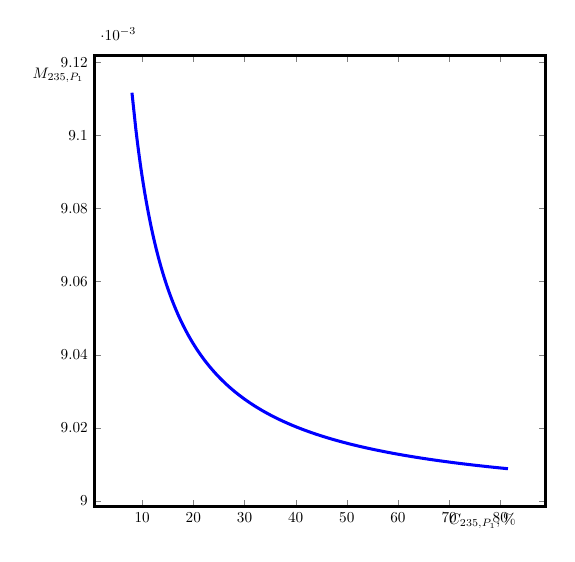
\begin{tikzpicture}[,
scale=0.55]
\begin{axis}[
  xlabel style = {{at={(axis description cs:.86,0)}}},
  ylabel = {$M_{235,P_1}$},
  ylabel style = {{at={(axis description cs:-0.08,.925)},rotate=270,anchor=south}},
  xlabel = {$C_{235,P_1}, \%$},
  width=12cm, height=12cm, line width=2pt
]

\addplot+[
  mark = {none}
] coordinates {
  (8.0, 0.009111645553414241)
  (8.75, 0.0091017702125065)
  (9.0, 0.009098848295071484)
  (9.25, 0.009096086045214)
  (9.5, 0.009093470723500143)
  (9.75, 0.009090990910644607)
  (10.0, 0.00908863634082525)
  (10.25, 0.009086397759630997)
  (10.5, 0.009084266802498001)
  (10.75, 0.009082235890267501)
  (11.0, 0.00908029813911642)
  (11.25, 0.009078447282604948)
  (11.5, 0.009076677603981013)
  (11.75, 0.009074983877200895)
  (12.0, 0.009073361315384259)
  (12.25, 0.00907180552563272)
  (12.5, 0.009070312469313927)
  (12.75, 0.009068878458541407)
  (13.0, 0.009067500000042155)
  (13.25, 0.009066173954411696)
  (13.5, 0.00906489728787538)
  (13.750000000000002, 0.009063667581395724)
  (14.000000000000002, 0.009062482014421195)
  (14.249999999999998, 0.009061338339251261)
  (14.499999999999998, 0.009060234375023613)
  (14.75, 0.009059168051505043)
  (15.0, 0.009058137545975231)
  (15.25, 0.00905714105051603)
  (15.5, 0.00905617690879367)
  (15.75, 0.009055243570310421)
  (16.0, 0.009054339582084164)
  (16.25, 0.00905346358110072)
  (16.5, 0.009052614287456559)
  (16.75, 0.009051790498119234)
  (17.0, 0.009050991081241673)
  (17.25, 0.00905021497097372)
  (17.5, 0.009049461162720995)
  (17.75, 0.009048728708806643)
  (18.0, 0.00904801671449666)
  (18.25, 0.009047324334353698)
  (18.5, 0.00904665076888807)
  (18.75, 0.009045995261478194)
  (19.0, 0.009045357095535361)
  (19.25, 0.009044735639730662)
  (19.5, 0.009044130154683458)
  (19.75, 0.009043540060440437)
  (20.0, 0.00904296481221043)
  (20.25, 0.009042403834595814)
  (20.5, 0.009041856609191412)
  (20.75, 0.00904132263216406)
  (21.0, 0.00904080143545228)
  (21.25, 0.009040292553237213)
  (21.5, 0.00903979550937721)
  (21.75, 0.009039309994501544)
  (22.0, 0.009038835564449479)
  (22.25, 0.009038371843888997)
  (22.5, 0.009037918474243971)
  (22.75, 0.009037475112769424)
  (23.0, 0.009037041431687414)
  (23.25, 0.009036617117378845)
  (23.5, 0.009036201869627142)
  (23.75, 0.009035795400909865)
  (24.0, 0.009035397435734786)
  (24.25, 0.009035007710017202)
  (24.5, 0.009034625970495555)
  (24.75, 0.00903425197418256)
  (25.0, 0.009033885487849455)
  (25.25, 0.009033526287540965)
  (25.5, 0.009033174158118945)
  (25.75, 0.009032828892832686)
  (26.0, 0.009032490292914117)
  (26.25, 0.009032158167196222)
  (26.5, 0.009031832331753151)
  (26.75, 0.009031512609560576)
  (27.0, 0.009031198830174978)
  (27.250000000000004, 0.009030890829430675)
  (27.500000000000004, 0.009030588449153424)
  (27.750000000000004, 0.009030291536889548)
  (28.000000000000004, 0.009029999945649653)
  (28.249999999999996, 0.009029713533665974)
  (28.499999999999996, 0.00902943216416257)
  (28.749999999999996, 0.009029155705137498)
  (28.999999999999996, 0.009028884029156364)
  (29.25, 0.009028617013156427)
  (29.5, 0.009028354538260753)
  (29.75, 0.009028096489601721)
  (30.0, 0.00902784275615345)
  (30.25, 0.009027593230572475)
  (30.5, 0.009027347809046375)
  (30.75, 0.009027106391149743)
  (31.0, 0.00902686887970717)
  (31.25, 0.009026635180662839)
  (31.5, 0.009026405202956339)
  (31.75, 0.009026178858404345)
  (32.0, 0.009025956061587903)
  (32.25, 0.009025736729744938)
  (32.5, 0.009025520782667745)
  (32.75, 0.009025308142605212)
  (33.0, 0.009025098734169474)
  (33.25, 0.009024892484246807)
  (33.5, 0.009024689321912506)
  (33.75, 0.009024489178349589)
  (34.0, 0.009024291986771057)
  (34.25, 0.009024097682345614)
  (34.5, 0.009023906202126574)
  (34.75, 0.009023717484983906)
  (35.0, 0.009023531471539137)
  (35.25, 0.009023348104103083)
  (35.5, 0.009023167326616195)
  (35.75, 0.009022989084591409)
  (36.0, 0.009022813325059406)
  (36.25, 0.009022639996516136)
  (36.5, 0.009022469048872474)
  (36.75, 0.009022300433405987)
  (37.0, 0.009022134102714624)
  (37.25, 0.0090219700106723)
  (37.5, 0.009021808112386228)
  (37.75, 0.009021648364155999)
  (38.0, 0.009021490723434238)
  (38.25, 0.009021335148788823)
  (38.5, 0.009021181599866602)
  (38.75, 0.009021030037358468)
  (39.0, 0.009020880422965822)
  (39.25, 0.009020732719368324)
  (39.5, 0.009020586890192831)
  (39.75, 0.00902044289998355)
  (40.0, 0.009020300714173297)
  (40.25, 0.009020160295716685)
  (40.5, 0.009020021613513425)
  (40.75, 0.009019884636650533)
  (41.0, 0.009019749333815445)
  (41.25, 0.009019615674453465)
  (41.5, 0.009019483628744707)
  (41.75, 0.009019353167581854)
  (42.0, 0.009019224262548657)
  (42.25, 0.009019096885899256)
  (42.5, 0.009018971010538156)
  (42.75, 0.009018846610000958)
  (43.0, 0.009018723658435686)
  (43.25, 0.009018602130584792)
  (43.5, 0.009018482001767763)
  (43.75, 0.009018363247864284)
  (44.0, 0.00901824584529798)
  (44.25, 0.009018129771020695)
  (44.5, 0.009018015002497262)
  (44.75, 0.00901790151769078)
  (45.0, 0.009017789295048354)
  (45.25, 0.009017678313487286)
  (45.5, 0.009017568552381682)
  (45.75, 0.009017459991549497)
  (46.0, 0.009017352611239942)
  (46.25, 0.009017246392121295)
  (46.5, 0.00901714131526906)
  (46.75, 0.009017037362154458)
  (47.0, 0.009016934514633253)
  (47.25, 0.009016832754934914)
  (47.5, 0.009016732065652023)
  (47.75, 0.009016633001095729)
  (48.0, 0.009016534446810474)
  (48.25, 0.009016436915934194)
  (48.5, 0.009016340392608286)
  (48.75, 0.009016244861300112)
  (49.0, 0.009016150306794668)
  (49.25, 0.009016056714186524)
  (49.5, 0.009015964068871979)
  (49.75, 0.009015872356541454)
  (50.0, 0.009015781563172147)
  (50.24999999999999, 0.00901569167502086)
  (50.5, 0.009015602678617089)
  (50.74999999999999, 0.009015514560756284)
  (51.0, 0.009015427308493298)
  (51.24999999999999, 0.009015340909136091)
  (51.5, 0.009015255350239526)
  (51.74999999999999, 0.009015170619599432)
  (52.0, 0.009015086705246778)
  (52.25, 0.009015003595442049)
  (52.5, 0.009014921278669761)
  (52.75, 0.00901483974363315)
  (53.0, 0.009014758979249004)
  (53.25, 0.009014678974642627)
  (53.5, 0.009014599719142978)
  (53.75, 0.009014521202277909)
  (54.0, 0.009014443413769559)
  (54.25, 0.009014366343529881)
  (54.50000000000001, 0.00901428998165625)
  (54.75, 0.009014214318427251)
  (55.00000000000001, 0.00901413934429854)
  (55.25, 0.009014065049898833)
  (55.50000000000001, 0.009013991426025996)
  (55.75, 0.009013918463643251)
  (56.00000000000001, 0.009013846153875479)
  (56.25, 0.009013774488005614)
  (56.49999999999999, 0.00901370345747114)
  (56.75, 0.009013633053860692)
  (56.99999999999999, 0.009013563268910726)
  (57.25, 0.009013494094502271)
  (57.49999999999999, 0.009013425522657811)
  (57.75, 0.00901335754553819)
  (57.99999999999999, 0.009013290155439639)
  (58.25, 0.009013223344790855)
  (58.5, 0.00901315710615017)
  (58.75, 0.009013091432202788)
  (59.0, 0.009013026315758083)
  (59.25, 0.00901296174974698)
  (59.5, 0.009012897727219393)
  (59.75, 0.009012834241341723)
  (60.0, 0.009012771285394442)
  (60.25, 0.009012708852769698)
  (60.5, 0.00901264693696901)
  (60.75000000000001, 0.009012585531601018)
  (61.0, 0.00901252463037926)
  (61.25000000000001, 0.009012464227120046)
  (61.5, 0.009012404315740343)
  (61.75000000000001, 0.009012344890255737)
  (62.0, 0.009012285944778433)
  (62.25000000000001, 0.009012227473515303)
  (62.5, 0.009012169470765989)
  (62.74999999999999, 0.009012111930921026)
  (63.0, 0.009012054848460052)
  (63.24999999999999, 0.00901199821795001)
  (63.5, 0.009011942034043426)
  (63.74999999999999, 0.009011886291476714)
  (64.0, 0.009011830985068525)
  (64.25, 0.009011776109718119)
  (64.5, 0.009011721660403788)
  (64.75, 0.009011667632181317)
  (65.0, 0.009011614020182456)
  (65.25, 0.009011560819613454)
  (65.5, 0.009011508025753606)
  (65.75, 0.00901145563395382)
  (66.0, 0.009011403639635264)
  (66.25, 0.009011352038287967)
  (66.5, 0.009011300825469516)
  (66.75, 0.00901124999680374)
  (67.0, 0.009011199547979423)
  (67.25, 0.00901114947474907)
  (67.5, 0.009011099772927661)
  (67.75, 0.009011050438391446)
  (68.0, 0.009011001467076764)
  (68.25, 0.00901095285497887)
  (68.5, 0.0090109045981508)
  (68.75, 0.009010856692702247)
  (69.0, 0.00901080913479844)
  (69.25, 0.009010761920659067)
  (69.5, 0.009010715046557203)
  (69.75, 0.009010668508818246)
  (70.0, 0.009010622303818869)
  (70.25, 0.00901057642798601)
  (70.5, 0.009010530877795835)
  (70.75, 0.00901048564977274)
  (71.0, 0.009010440740488368)
  (71.25, 0.009010396146560597)
  (71.5, 0.009010351864652596)
  (71.75, 0.009010307891471833)
  (72.0, 0.009010264223769117)
  (72.25, 0.009010220858337654)
  (72.5, 0.009010177792012079)
  (72.75, 0.00901013502166751)
  (73.0, 0.00901009254421861)
  (73.25, 0.009010050356618626)
  (73.5, 0.009010008455858446)
  (73.75, 0.009009966838965653)
  (74.0, 0.009009925503003568)
  (74.25, 0.009009884445070285)
  (74.5, 0.009009843662297713)
  (74.75, 0.009009803151850605)
  (75.0, 0.009009762910925562)
  (75.25, 0.00900972293675004)
  (75.5, 0.009009683226581354)
  (75.75, 0.009009643777705635)
  (76.0, 0.009009604587436796)
  (76.25, 0.009009565653115467)
  (76.5, 0.009009526972107914)
  (76.75, 0.00900948854180492)
  (77.0, 0.009009450359620655)
  (77.25, 0.009009412422991511)
  (77.5, 0.0090093747293749)
  (77.75, 0.009009337276248005)
  (78.0, 0.009009300061106531)
  (78.25, 0.009009263431930687)
  (78.5, 0.009009226717816872)
  (78.75, 0.009009190241608116)
  (79.0, 0.009009153717338046)
  (79.25, 0.009009117547127953)
  (79.5, 0.009009081533171134)
  (79.75, 0.009009046608607772)
  (80.0, 0.009009011263082943)
  (80.25, 0.009008976130382018)
  (80.5, 0.009008941231325876)
  (80.75, 0.009008905699671515)
  (81.0, 0.009008871149798441)
  (81.25, 0.009008836806363333)
  (81.5, 0.009008802666955288)
};

\end{axis}
\end{tikzpicture}

}
%     \caption{{Зависимость массы $^{235}$U в потоке обогащенной фракции первого каскада $P_1$ от концентрации $^{235}$U в потоке легкой фракции первого каскада{\label{M235P1}}}}
% \end{figure}



% \begin{figure}
%     \centering
%     \begin{minipage}{.5\textwidth}
%       \centering
%       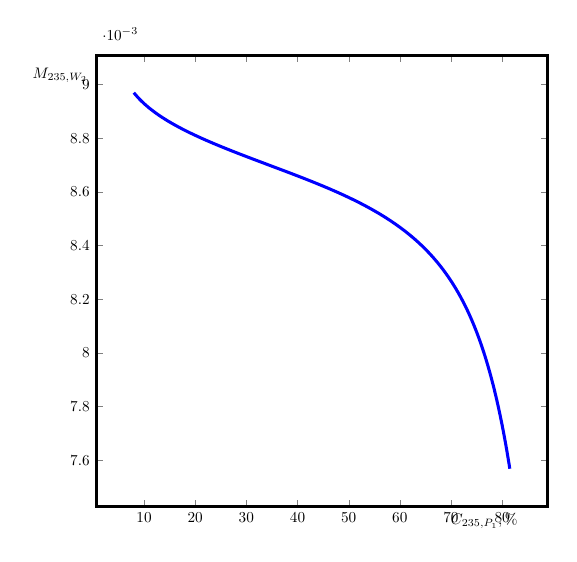
\begin{tikzpicture}[,
scale=0.55]
\begin{axis}[
  xlabel style = {{at={(axis description cs:.86,0)}}},
  ylabel = {$M_{235,W_2}$},
  ylabel style = {{at={(axis description cs:-0.08,.925)},rotate=270,anchor=south}},
  xlabel = {$C_{235,P_1}, \%$},
  width=12cm, height=12cm, line width=2pt
]

\addplot+[
  mark = {none}
] coordinates {
  (8.0, 0.008969582934887354)
  (8.75, 0.008953050957470687)
  (9.0, 0.008947961457989935)
  (9.25, 0.008943055236043482)
  (9.5, 0.008938318351511982)
  (9.75, 0.008933738550573236)
  (10.0, 0.008929304579336527)
  (10.25, 0.00892500600276735)
  (10.5, 0.008920834068883481)
  (10.75, 0.008916780111045451)
  (11.0, 0.008912836522459945)
  (11.25, 0.00890899638778039)
  (11.5, 0.008905253328491191)
  (11.75, 0.00890160156292447)
  (12.0, 0.008898035595833407)
  (12.25, 0.008894550529189556)
  (12.5, 0.008891142055842764)
  (12.75, 0.008887805346784065)
  (13.0, 0.00888453702453666)
  (13.25, 0.00888133327101651)
  (13.5, 0.008878190722767425)
  (13.750000000000002, 0.008875106482081157)
  (14.000000000000002, 0.008872077308430648)
  (14.249999999999998, 0.008869100608211533)
  (14.499999999999998, 0.008866173925463825)
  (14.75, 0.008863294824375137)
  (15.0, 0.00886046103386761)
  (15.25, 0.008857670643016527)
  (15.5, 0.0088549215481551)
  (15.75, 0.008852211964820795)
  (16.0, 0.008849540023391618)
  (16.25, 0.00884690431436794)
  (16.5, 0.008844303237468832)
  (16.75, 0.008841735275167406)
  (17.0, 0.008839199039822518)
  (17.25, 0.008836693480195931)
  (17.5, 0.00883421697699065)
  (17.75, 0.0088317687332981)
  (18.0, 0.00882934748342718)
  (18.25, 0.00882695214685525)
  (18.5, 0.008824581764264412)
  (18.75, 0.008822235354809235)
  (19.0, 0.008819912216795097)
  (19.25, 0.00881761123796545)
  (19.5, 0.008815331753722773)
  (19.75, 0.00881307281029624)
  (20.0, 0.008810833888339926)
  (20.25, 0.008808614074903603)
  (20.5, 0.008806412834731561)
  (20.75, 0.008804229443483637)
  (21.0, 0.008802063270662694)
  (21.25, 0.008799913744817398)
  (21.5, 0.00879778027046047)
  (21.75, 0.008795662265158915)
  (22.0, 0.008793559276179001)
  (22.25, 0.00879147051686481)
  (22.5, 0.008789395993835127)
  (22.75, 0.008787334812847844)
  (23.0, 0.008785286700981111)
  (23.25, 0.008783251073485748)
  (23.5, 0.008781227661490464)
  (23.75, 0.008779215933748342)
  (24.0, 0.008777215454272918)
  (24.25, 0.008775225876559527)
  (24.5, 0.008773246979830614)
  (24.75, 0.008771278510945961)
  (25.0, 0.008769319200942987)
  (25.25, 0.008767369764545823)
  (25.5, 0.008765429352778268)
  (25.75, 0.008763497724964686)
  (26.0, 0.00876157460680785)
  (26.25, 0.008759659733538669)
  (26.5, 0.008757752721138398)
  (26.75, 0.008755853183943181)
  (27.0, 0.008753960981176848)
  (27.250000000000004, 0.008752075704564152)
  (27.500000000000004, 0.008750197251064693)
  (27.750000000000004, 0.008748325098700112)
  (28.000000000000004, 0.008746459143606207)
  (28.249999999999996, 0.008744599156599683)
  (28.499999999999996, 0.00874274475756152)
  (28.749999999999996, 0.00874089570432083)
  (28.999999999999996, 0.008739051758361226)
  (29.25, 0.008737212859217611)
  (29.5, 0.008735378568265433)
  (29.75, 0.008733548658001515)
  (30.0, 0.008731722851187139)
  (30.25, 0.008729901060330605)
  (30.5, 0.008728082992807404)
  (30.75, 0.008726268277156625)
  (31.0, 0.008724456956166039)
  (31.25, 0.008722648537674339)
  (31.5, 0.00872084298824132)
  (31.75, 0.008719039917813124)
  (32.0, 0.008717239389980553)
  (32.25, 0.008715440946923838)
  (32.5, 0.008713644358357074)
  (32.75, 0.008711849635932507)
  (33.0, 0.00871005612709628)
  (33.25, 0.008708264214899087)
  (33.5, 0.00870647327897643)
  (33.75, 0.008704683167840163)
  (34.0, 0.008702893749631745)
  (34.25, 0.008701104753714752)
  (34.5, 0.008699315918146305)
  (34.75, 0.008697527280060588)
  (35.0, 0.008695738295444984)
  (35.25, 0.008693949011086596)
  (35.5, 0.008692159067325417)
  (35.75, 0.008690368279467689)
  (36.0, 0.008688576444007815)
  (36.25, 0.008686783394698666)
  (36.5, 0.008684988871695434)
  (36.75, 0.008683192626879025)
  (37.0, 0.008681394560566527)
  (37.25, 0.008679594405661325)
  (37.5, 0.008677791839637863)
  (37.75, 0.00867598678009571)
  (38.0, 0.008674178926183503)
  (38.25, 0.008672368153057894)
  (38.5, 0.008670554088754482)
  (38.75, 0.0086687365946658)
  (39.0, 0.008666915421462824)
  (39.25, 0.008665090385095373)
  (39.5, 0.008663261262198822)
  (39.75, 0.008661427825532907)
  (40.0, 0.008659589749934544)
  (40.25, 0.008657746844634986)
  (40.5, 0.008655898846421654)
  (40.75, 0.00865404564337099)
  (41.0, 0.008652186658828356)
  (41.25, 0.008650322200803322)
  (41.5, 0.008648451545630592)
  (41.75, 0.008646574533356776)
  (42.0, 0.008644690955891309)
  (42.25, 0.008642800636894704)
  (42.5, 0.008640903224070825)
  (42.75, 0.00863899844671149)
  (43.0, 0.008637085957510716)
  (43.25, 0.00863516575727924)
  (43.5, 0.008633237218089401)
  (43.75, 0.008631300408230349)
  (44.0, 0.008629354764905747)
  (44.25, 0.008627400106242656)
  (44.5, 0.008625436177556048)
  (44.75, 0.0086234625877378)
  (45.0, 0.00862147908941806)
  (45.25, 0.008619485381956294)
  (45.5, 0.008617481036809113)
  (45.75, 0.008615465921339726)
  (46.0, 0.008613439478955834)
  (46.25, 0.008611401795773408)
  (46.5, 0.008609352102023984)
  (46.75, 0.008607290031975672)
  (47.0, 0.008605215642082472)
  (47.25, 0.008603128259590765)
  (47.5, 0.008601027675848224)
  (47.75, 0.008598913983259165)
  (48.0, 0.008596785691386668)
  (48.25, 0.008594643293756862)
  (48.5, 0.008592485759095589)
  (48.75, 0.008590313355086041)
  (49.0, 0.0085881251954436)
  (49.25, 0.008585921074581795)
  (49.5, 0.008583700611067892)
  (49.75, 0.008581463263063322)
  (50.0, 0.008579208603379272)
  (50.24999999999999, 0.008576936252814263)
  (50.5, 0.008574645722361236)
  (50.74999999999999, 0.008572336531763418)
  (51.0, 0.008570008133297382)
  (51.24999999999999, 0.00856766010981354)
  (51.5, 0.008565291973522108)
  (51.74999999999999, 0.008562903220451633)
  (52.0, 0.008560493278454286)
  (52.25, 0.00855806152083667)
  (52.5, 0.0085556076484768)
  (52.75, 0.008553130961714709)
  (53.0, 0.008550630846209386)
  (53.25, 0.00854810706771584)
  (53.5, 0.00854555774925702)
  (53.75, 0.0085429838369619)
  (54.0, 0.008540383924706487)
  (54.25, 0.008537757588306388)
  (54.50000000000001, 0.008535104091081134)
  (54.75, 0.008532422651702221)
  (55.00000000000001, 0.008529712611513763)
  (55.25, 0.008526973112919355)
  (55.50000000000001, 0.008524203723571044)
  (55.75, 0.008521403545945452)
  (56.00000000000001, 0.008518571606366723)
  (56.25, 0.00851570727763321)
  (56.49999999999999, 0.008512809808569574)
  (56.75, 0.008509878155889035)
  (56.99999999999999, 0.008506911456068385)
  (57.25, 0.008503908792779345)
  (57.49999999999999, 0.00850086938251702)
  (57.75, 0.008497792179323343)
  (57.99999999999999, 0.008494676202933862)
  (58.25, 0.008491520141475806)
  (58.5, 0.008488323553930758)
  (58.75, 0.008485084979440822)
  (59.0, 0.008481803250545655)
  (59.25, 0.008478477351644427)
  (59.5, 0.008475105879196487)
  (59.75, 0.008471688048711791)
  (60.0, 0.008468222192560626)
  (60.25, 0.008464707099481916)
  (60.5, 0.00846114133577974)
  (60.75000000000001, 0.008457523922427972)
  (61.0, 0.008453852639556711)
  (61.25000000000001, 0.00845012688494179)
  (61.5, 0.008446344688200533)
  (61.75000000000001, 0.008442504246032677)
  (62.0, 0.008438604167544233)
  (62.25000000000001, 0.008434642701742214)
  (62.5, 0.00843061819667875)
  (62.74999999999999, 0.008426528551434788)
  (63.0, 0.008422371991251038)
  (63.24999999999999, 0.008418146665359498)
  (63.5, 0.008413850388432755)
  (63.74999999999999, 0.008409481193270963)
  (64.0, 0.00840503667489769)
  (64.25, 0.008400514684896585)
  (64.5, 0.00839591280165317)
  (64.75, 0.008391228646229737)
  (65.0, 0.008386459646753221)
  (65.25, 0.008381602891968784)
  (65.5, 0.008376656246177845)
  (65.75, 0.008371616339520984)
  (66.0, 0.008366480231628762)
  (66.25, 0.008361245162791847)
  (66.5, 0.008355907301054039)
  (66.75, 0.00835046404896195)
  (67.0, 0.008344911421099945)
  (67.25, 0.008339246074549682)
  (67.5, 0.008333463823960592)
  (67.75, 0.008327561384019997)
  (68.0, 0.008321533879538923)
  (68.25, 0.00831537758511544)
  (68.5, 0.00830908814223659)
  (68.75, 0.008302660204893444)
  (69.0, 0.008296089646192446)
  (69.25, 0.00828937113819764)
  (69.5, 0.008282499224605326)
  (69.75, 0.008275468531667402)
  (70.0, 0.00826827347415231)
  (70.25, 0.008260908009095722)
  (70.5, 0.00825336596088543)
  (70.75, 0.008245640203393603)
  (71.0, 0.008237724568319199)
  (71.25, 0.00822961154384384)
  (71.5, 0.008221293669866929)
  (71.75, 0.00821276338124383)
  (72.0, 0.008204012187817605)
  (72.25, 0.00819503168306494)
  (72.5, 0.008185813088394164)
  (72.75, 0.008176346645735303)
  (73.0, 0.00816662305461966)
  (73.25, 0.008156631890100853)
  (73.5, 0.008146362682047308)
  (73.75, 0.008135803206441633)
  (74.0, 0.008124942750070615)
  (74.25, 0.008113768797907307)
  (74.5, 0.008102268366638297)
  (74.75, 0.00809042809718903)
  (75.0, 0.008078233643784233)
  (75.25, 0.008065670407119764)
  (75.5, 0.008052722827568548)
  (75.75, 0.008039374511333873)
  (76.0, 0.00802560836493737)
  (76.25, 0.008011406404869104)
  (76.5, 0.007996750206473837)
  (76.75, 0.00798161953598353)
  (77.0, 0.007965994104478175)
  (77.25, 0.007949851853015227)
  (77.5, 0.007933169944668625)
  (77.75, 0.007915923760480153)
  (78.0, 0.007898088701745708)
  (78.25, 0.007879637419106009)
  (78.5, 0.00786054173728438)
  (78.75, 0.007840771975822277)
  (79.0, 0.00782029584895143)
  (79.25, 0.0077990811576082175)
  (79.5, 0.007777091914924569)
  (79.75, 0.00775429154132833)
  (80.0, 0.007730640361314449)
  (80.25, 0.007706093308217856)
  (80.5, 0.00768060886945932)
  (80.75, 0.007654137404335572)
  (81.0, 0.007626629210857389)
  (81.25, 0.007598029377462495)
  (81.5, 0.00756827981297914)
};

\end{axis}
\end{tikzpicture}


% \caption{{Зависимость массы $^{235}$U в потоке тяжелой фракции второго каскада $W_2$ от концентрации $^{235}$U в потоке легкой фракции первого каскада{\label{M235W2}}}}
%     \end{minipage}%
%     \begin{minipage}{.5\textwidth}
%       \centering
%       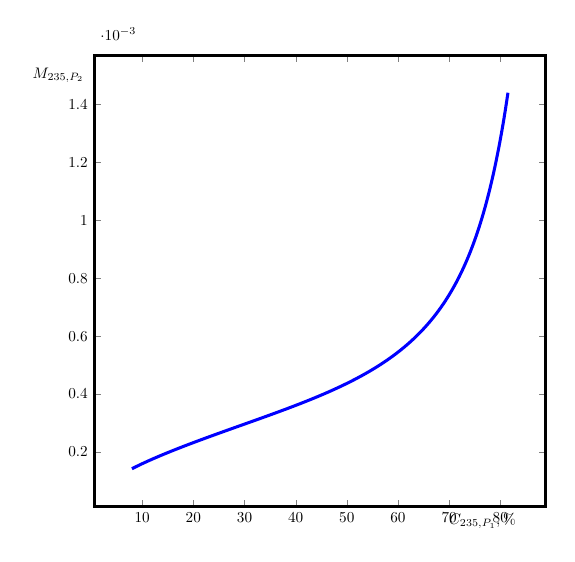
\begin{tikzpicture}[,
scale=0.55]
\begin{axis}[
  xlabel style = {{at={(axis description cs:.86,0)}}},
  ylabel = {$M_{235,P_2}$},
  ylabel style = {{at={(axis description cs:-0.08,.925)},rotate=270,anchor=south}},
  xlabel = {$C_{235,P_1}, \%$},
  width=12cm, height=12cm, line width=2pt
]

\addplot+[
  mark = {none}
] coordinates {
  (8.0, 0.00014206261852688643)
  (8.75, 0.0001487192550358152)
  (9.0, 0.00015088683708154766)
  (9.25, 0.00015303080917051723)
  (9.5, 0.0001551523719881621)
  (9.75, 0.00015725236007136956)
  (10.0, 0.0001593317614887236)
  (10.25, 0.00016139175686364607)
  (10.5, 0.00016343273361451926)
  (10.75, 0.0001654557792220484)
  (11.0, 0.0001674616166564755)
  (11.25, 0.00016945089482455766)
  (11.5, 0.00017142427548982213)
  (11.75, 0.00017338231427642395)
  (12.0, 0.00017532571955085064)
  (12.25, 0.00017725499644316329)
  (12.5, 0.00017917041347116197)
  (12.75, 0.00018107311175734472)
  (13.0, 0.00018296297550549672)
  (13.25, 0.00018484068339518633)
  (13.5, 0.00018670656510795378)
  (13.750000000000002, 0.00018856109931456714)
  (14.000000000000002, 0.00019040470599054806)
  (14.249999999999998, 0.00019223773103972837)
  (14.499999999999998, 0.00019406044955978683)
  (14.75, 0.00019587322712990587)
  (15.0, 0.00019767651210762089)
  (15.25, 0.00019947040749950323)
  (15.5, 0.0002012553606385691)
  (15.75, 0.000203031605489627)
  (16.0, 0.0002047995586925459)
  (16.25, 0.00020655926673278035)
  (16.5, 0.00020831104998772658)
  (16.75, 0.00021005522295182956)
  (17.0, 0.00021179204141915403)
  (17.25, 0.00021352149077778944)
  (17.5, 0.00021524418573034358)
  (17.75, 0.00021695997550854248)
  (18.0, 0.00021866923106948102)
  (18.25, 0.00022037218749844817)
  (18.5, 0.0002220690046236574)
  (18.75, 0.00022375990666895904)
  (19.0, 0.00022544487874026487)
  (19.25, 0.00022712440176520985)
  (19.5, 0.000228798400960687)
  (19.75, 0.0002304672501441958)
  (20.0, 0.00023213092387050163)
  (20.25, 0.00023378975969221073)
  (20.5, 0.00023544377445984787)
  (20.75, 0.00023709318868042308)
  (21.0, 0.00023873816478958473)
  (21.25, 0.00024037880841981435)
  (21.5, 0.0002420152389167409)
  (21.75, 0.0002436477293426275)
  (22.0, 0.00024527628827047715)
  (22.25, 0.00024690132702418757)
  (22.5, 0.000248522480408844)
  (22.75, 0.0002501402999215804)
  (23.0, 0.00025175473070630355)
  (23.25, 0.00025336604389309693)
  (23.5, 0.00025497420813668046)
  (23.75, 0.0002565794671615227)
  (24.0, 0.00025818198146186926)
  (24.25, 0.00025978183345767603)
  (24.5, 0.00026137899066494216)
  (24.75, 0.00026297346323659904)
  (25.0, 0.00026456628690646705)
  (25.25, 0.0002661565229951418)
  (25.5, 0.0002677448053406744)
  (25.75, 0.000269331167867999)
  (26.0, 0.0002709156861062661)
  (26.25, 0.00027249843365755483)
  (26.5, 0.0002740796106147544)
  (26.75, 0.00027565942561739483)
  (27.0, 0.00027723784899813124)
  (27.250000000000004, 0.0002788151248665254)
  (27.500000000000004, 0.0002803911980887289)
  (27.750000000000004, 0.0002819664381894382)
  (28.000000000000004, 0.00028354080204344467)
  (28.249999999999996, 0.00028511437706629176)
  (28.499999999999996, 0.0002866874066010505)
  (28.749999999999996, 0.00028826000081666806)
  (28.999999999999996, 0.00028983227079514023)
  (29.25, 0.00029140415393881665)
  (29.5, 0.00029297596999531867)
  (29.75, 0.0002945478316002078)
  (30.0, 0.00029611990496630937)
  (30.25, 0.0002976921702418694)
  (30.5, 0.00029926481623896936)
  (30.75, 0.00030083811399311594)
  (31.0, 0.0003024119235411315)
  (31.25, 0.0003039866429885015)
  (31.5, 0.00030556221471501877)
  (31.75, 0.0003071389405912217)
  (32.0, 0.00030871667160734965)
  (32.25, 0.0003102957828210971)
  (32.5, 0.00031187642431066976)
  (32.75, 0.00031345850667270484)
  (33.0, 0.0003150426070731949)
  (33.25, 0.0003166282693477201)
  (33.5, 0.00031821604293607675)
  (33.75, 0.00031980601050942775)
  (34.0, 0.0003213982371393116)
  (34.25, 0.00032299292863086315)
  (34.5, 0.00032459028398027255)
  (34.75, 0.0003261902049233192)
  (35.0, 0.0003277931760941529)
  (35.25, 0.0003293990930164905)
  (35.5, 0.0003310082592907783)
  (35.75, 0.00033262080512371883)
  (36.0, 0.0003342368810515949)
  (36.25, 0.00033585660181746966)
  (36.5, 0.0003374801771770407)
  (36.75, 0.00033910780652696257)
  (37.0, 0.0003407395421480962)
  (37.25, 0.0003423756050109775)
  (37.5, 0.0003440162727483667)
  (37.75, 0.0003456615840602884)
  (38.0, 0.00034731179725073575)
  (38.25, 0.00034896699573092933)
  (38.5, 0.0003506275111121188)
  (38.75, 0.0003522934426926643)
  (39.0, 0.00035396500150299795)
  (39.25, 0.0003556423342729505)
  (39.5, 0.0003573256279940082)
  (39.75, 0.00035901507445064196)
  (40.0, 0.0003607109642387537)
  (40.25, 0.0003624134510816995)
  (40.5, 0.00036412276709177246)
  (40.75, 0.0003658389932795444)
  (41.0, 0.0003675626749870876)
  (41.25, 0.00036929347365014225)
  (41.5, 0.00037103208311411453)
  (41.75, 0.00037277863422507766)
  (42.0, 0.00037453330665735036)
  (42.25, 0.0003762962490045512)
  (42.5, 0.00037806778646733223)
  (42.75, 0.00037984816328946784)
  (43.0, 0.0003816377009249703)
  (43.25, 0.00038343637330555364)
  (43.5, 0.0003852447836783621)
  (43.75, 0.0003870628396339368)
  (44.0, 0.0003888910803922337)
  (44.25, 0.00039072966477804054)
  (44.5, 0.0003925788249412114)
  (44.75, 0.0003944389299529779)
  (45.0, 0.000396310205630296)
  (45.25, 0.00039819293153099146)
  (45.5, 0.00040008751557256785)
  (45.75, 0.00040199407020977)
  (46.0, 0.00040391313228410814)
  (46.25, 0.0004058445963478875)
  (46.5, 0.000407789213245078)
  (46.75, 0.00040974733017878527)
  (47.0, 0.00041171887255078395)
  (47.25, 0.00041370449534414876)
  (47.5, 0.00041570438980380016)
  (47.75, 0.0004177190178365665)
  (48.0, 0.00041974875542380533)
  (48.25, 0.00042179362217733245)
  (48.5, 0.00042385463351269574)
  (48.75, 0.0004259315062140724)
  (49.0, 0.00042802511135106775)
  (49.25, 0.0004301356396047288)
  (49.5, 0.0004322634578040857)
  (49.75, 0.00043440909347813053)
  (50.0, 0.0004365729597928729)
  (50.24999999999999, 0.00043875542220659535)
  (50.5, 0.00044095695625585315)
  (50.74999999999999, 0.0004431780289928668)
  (51.0, 0.00044541917519591665)
  (51.24999999999999, 0.00044768079932255096)
  (51.5, 0.0004499633767174201)
  (51.74999999999999, 0.0004522673991477988)
  (52.0, 0.00045459342679249256)
  (52.25, 0.00045694207460538074)
  (52.5, 0.00045931363019295965)
  (52.75, 0.0004617087819184397)
  (53.0, 0.0004641281330396219)
  (53.25, 0.00046657190692678724)
  (53.5, 0.0004690419698859583)
  (53.75, 0.00047153736531601004)
  (54.0, 0.00047405948906307284)
  (54.25, 0.00047660875522349496)
  (54.50000000000001, 0.0004791858905751159)
  (54.75, 0.00048179166672502986)
  (55.00000000000001, 0.00048442673278477555)
  (55.25, 0.00048709193697948)
  (55.50000000000001, 0.0004897877024549516)
  (55.75, 0.0004925149176977991)
  (56.00000000000001, 0.0004952745475087547)
  (56.25, 0.000498067210372404)
  (56.49999999999999, 0.0005008936489015665)
  (56.75, 0.0005037548979716578)
  (56.99999999999999, 0.0005066518128423399)
  (57.25, 0.0005095853017229255)
  (57.49999999999999, 0.0005125561401407897)
  (57.75, 0.0005155653662148463)
  (57.99999999999999, 0.0005186139525057761)
  (58.25, 0.0005217032033150501)
  (58.5, 0.0005248335522194126)
  (58.75, 0.0005280064527619661)
  (59.0, 0.0005312230652124307)
  (59.25, 0.0005344843981025534)
  (59.5, 0.000537791848022905)
  (59.75, 0.0005411461926299319)
  (60.0, 0.0005445490928338145)
  (60.25, 0.0005480017532877826)
  (60.5, 0.0005515056011892717)
  (60.75000000000001, 0.0005550616091730453)
  (61.0, 0.0005586719908225494)
  (61.25000000000001, 0.0005623373421782563)
  (61.5, 0.0005660596275398105)
  (61.75000000000001, 0.0005698406442230616)
  (62.0, 0.0005736817772341985)
  (62.25000000000001, 0.0005775847717730899)
  (62.5, 0.0005815512740872374)
  (62.74999999999999, 0.000585583379486238)
  (63.0, 0.000589682857209016)
  (63.24999999999999, 0.0005938515525905125)
  (63.5, 0.0005980916456106702)
  (63.74999999999999, 0.00060240509820575)
  (64.0, 0.0006067943101708379)
  (64.25, 0.0006112614248215335)
  (64.5, 0.0006158088587506189)
  (64.75, 0.0006204389859515801)
  (65.0, 0.0006251543734292362)
  (65.25, 0.0006299579276446713)
  (65.5, 0.000634851779575759)
  (65.75, 0.0006398392944328368)
  (66.0, 0.0006449234080065024)
  (66.25, 0.0006501068754961208)
  (66.5, 0.0006553935244154773)
  (66.75, 0.0006607859478417916)
  (67.0, 0.0006662881268794789)
  (67.25, 0.0006719034001993863)
  (67.5, 0.0006776359489670697)
  (67.75, 0.0006834890543714472)
  (68.0, 0.0006894675875378399)
  (68.25, 0.000695575269863432)
  (68.5, 0.0007018164559142097)
  (68.75, 0.000708196487808803)
  (69.0, 0.0007147194886059934)
  (69.25, 0.0007213907824614268)
  (69.5, 0.0007282158219518746)
  (69.75, 0.0007351999771508405)
  (70.0, 0.0007423488296665546)
  (70.25, 0.0007496684188902872)
  (70.5, 0.0007571649169104045)
  (70.75, 0.0007648454463791348)
  (71.0, 0.0007727161721691653)
  (71.25, 0.0007807846027167577)
  (71.5, 0.0007890581947856685)
  (71.75, 0.0007975445102280024)
  (72.0, 0.0008062520359515104)
  (72.25, 0.000815189175272715)
  (72.5, 0.0008243647036179145)
  (72.75, 0.0008337883759322068)
  (73.0, 0.0008434694895989494)
  (73.25, 0.0008534184665177729)
  (73.5, 0.000863645773811138)
  (73.75, 0.0008741636325240199)
  (74.0, 0.0008849827529329532)
  (74.25, 0.0008961156471629762)
  (74.5, 0.0009075752956594171)
  (74.75, 0.0009193750546615769)
  (75.0, 0.0009315292671413294)
  (75.25, 0.0009440525296302777)
  (75.5, 0.0009569603990128037)
  (75.75, 0.0009702692663717642)
  (76.0, 0.000983996222499424)
  (76.25, 0.0009981592482463631)
  (76.5, 0.001012776765634078)
  (76.75, 0.0010278690058213892)
  (77.0, 0.0010434562551424789)
  (77.25, 0.0010595605699762838)
  (77.5, 0.0010762047847062738)
  (77.75, 0.0010934135157678515)
  (78.0, 0.0011112113593608204)
  (78.25, 0.0011296260128246794)
  (78.5, 0.0011486849805324923)
  (78.75, 0.0011684182657858363)
  (79.0, 0.0011888578683866158)
  (79.25, 0.001210036389519737)
  (79.5, 0.0012319896182465644)
  (79.75, 0.0012547550672794418)
  (80.0, 0.0012783709017684958)
  (80.25, 0.001302882822164161)
  (80.5, 0.0013283323618665562)
  (80.75, 0.0013547682953359422)
  (81.0, 0.0013822419389410525)
  (81.25, 0.0014108074289008383)
  (81.5, 0.0014405228539761475)
};

\end{axis}
\end{tikzpicture}


% \caption{{Зависимость массы $^{235}$U в потоке легкой фракции второго каскада $P_2$ от концентрации $^{235}$U в потоке легкой фракции первого каскада{\label{M235P2}}}}
% \end{minipage}
% \end{figure}





% \begin{figure}
%     \centering
%     \begin{minipage}{.5\textwidth}
%       \centering
%       \input{images/tex/loop_0.0495}
% \caption{{Зависимость массы $^{235}$U в потоке тяжелой фракции второго каскада $W_2$ от концентрации $^{235}$U в потоке легкой фракции первого каскада{\label{M235W2}}}}
%     \end{minipage}%
%     \begin{minipage}{.5\textwidth}
%       \centering
%       \input{images/tex/loop_0.0495}
% \caption{{Зависимость массы $^{235}$U в потоке легкой фракции второго каскада $P_2$ от концентрации $^{235}$U в потоке легкой фракции первого каскада{\label{M235P2}}}}
% \end{minipage}
% \end{figure}



% \clearpage


% \begin{figure}
%     \centerfloat{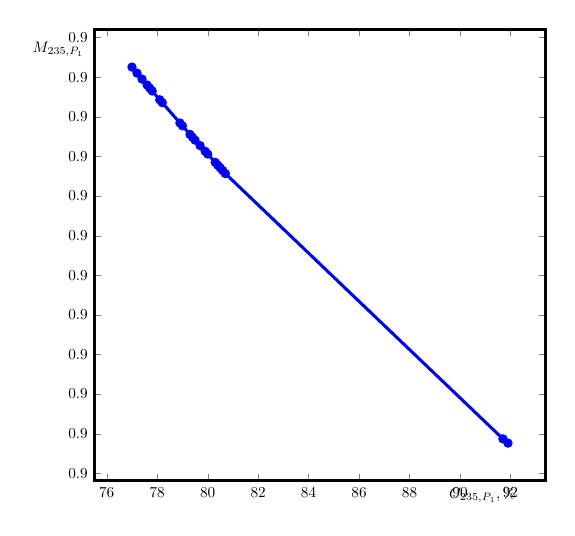
\begin{tikzpicture}[,
scale=0.55]
\begin{axis}[
  xlabel style = {{at={(axis description cs:.86,0)}}},
  ylabel = {$M_{235,P_1}$},
  ylabel style = {{at={(axis description cs:-0.08,.925)},rotate=270,anchor=south}},
  xlabel = {$C_{235,P_1}, \%$},
  width=12cm, height=12cm, line width=2pt
]

\addplot+ coordinates {
  (77.0, 0.9009450359620654)
  (77.2, 0.9009419990795269)
  (77.4, 0.9009389777821928)
  (77.60000000000001, 0.9009359719406014)
  (77.7, 0.9009344747754668)
  (77.8, 0.90093298142607)
  (78.10000000000001, 0.9009285241128198)
  (78.2, 0.9009270802954181)
  (78.9, 0.9009168234481284)
  (79.0, 0.9009153717338045)
  (79.3, 0.9009110332650255)
  (79.4, 0.9009095921620832)
  (79.5, 0.9009081533171134)
  (79.7, 0.9009053704589045)
  (79.9, 0.9009025375084988)
  (80.0, 0.9009011263082943)
  (80.30000000000001, 0.9008969131373471)
  (80.4, 0.9008955159491712)
  (80.5, 0.9008941231325875)
  (80.60000000000001, 0.9008927329166118)
  (80.7, 0.9008912634630402)
  (91.7, 0.9007572870913582)
  (91.9, 0.9007551470285345)
};


\end{axis}
\end{tikzpicture}

}
%     \caption{{Зависимость массы $^{235}$U в потоке обогащенной фракции первого каскада $P_1$ от концентрации $^{235}$U в потоке легкой фракции первого каскада{\label{M235P1}}}}
% \end{figure}



% \begin{figure}
%     \centering
%     \begin{minipage}{.5\textwidth}
%       \centering
%       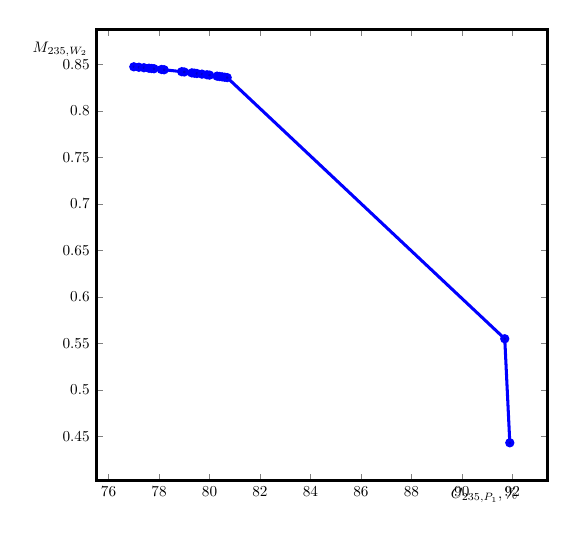
\begin{tikzpicture}[,
scale=0.55]
\begin{axis}[
  xlabel style = {{at={(axis description cs:.86,0)}}},
  ylabel = {$M_{235,W_2}$},
  ylabel style = {{at={(axis description cs:-0.08,.925)},rotate=270,anchor=south}},
  xlabel = {$C_{235,P_1}, \%$},
  width=12cm, height=12cm, line width=2pt
]

\addplot+ coordinates {
  (77.0, 0.847255489119533)
  (77.2, 0.8467603241080492)
  (77.4, 0.8462531188165721)
  (77.60000000000001, 0.8457329675283174)
  (77.7, 0.8454679156671182)
  (77.8, 0.8451994563533017)
  (78.10000000000001, 0.844373436959269)
  (78.2, 0.8440912014568814)
  (78.9, 0.8420078814549162)
  (79.0, 0.8416940899299918)
  (79.3, 0.8407279531588767)
  (79.4, 0.8403970353687986)
  (79.5, 0.8400617608739249)
  (79.7, 0.8393771028845441)
  (79.9, 0.8386732864869232)
  (80.0, 0.8383142216959854)
  (80.30000000000001, 0.8372059387814224)
  (80.4, 0.8368260037593748)
  (80.5, 0.8364406357319992)
  (80.60000000000001, 0.8360497907477974)
  (80.7, 0.8356532251113954)
  (91.7, 0.5548271981035123)
  (91.9, 0.44298000135762333)
};

\end{axis}
\end{tikzpicture}


% \caption{{Зависимость массы $^{235}$U в потоке тяжелой фракции второго каскада $W_2$ от концентрации $^{235}$U в потоке легкой фракции первого каскада{\label{M235W2}}}}
%     \end{minipage}%
%     \begin{minipage}{.5\textwidth}
%       \centering
%       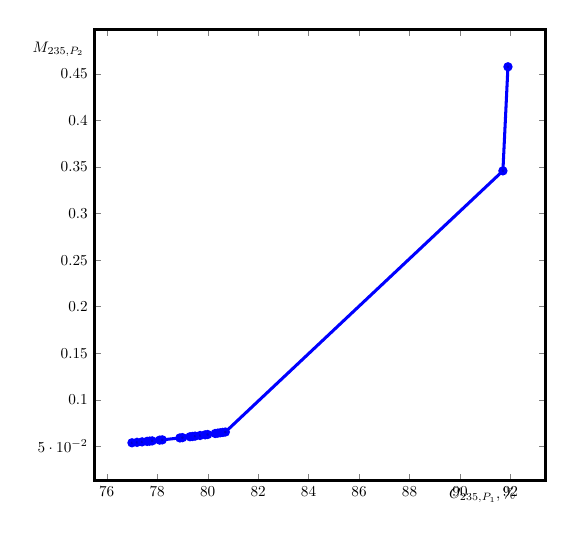
\begin{tikzpicture}[,
scale=0.55]
\begin{axis}[
  xlabel style = {{at={(axis description cs:.86,0)}}},
  ylabel = {$M_{235,P_2}$},
  ylabel style = {{at={(axis description cs:-0.08,.925)},rotate=270,anchor=south}},
  xlabel = {$C_{235,P_1}, \%$},
  width=12cm, height=12cm, line width=2pt
]

\addplot+ coordinates {
  (77.0, 0.05368954684253237)
  (77.2, 0.054181674971477814)
  (77.4, 0.054685858965620754)
  (77.60000000000001, 0.05520300441228407)
  (77.7, 0.0554665591083487)
  (77.8, 0.055733525072768485)
  (78.10000000000001, 0.05655508715355083)
  (78.2, 0.05683587883853662)
  (78.9, 0.058908941993212095)
  (79.0, 0.05922128180381264)
  (79.3, 0.06018308010614907)
  (79.4, 0.06051255679328454)
  (79.5, 0.060846392443188346)
  (79.7, 0.061528267574360626)
  (79.9, 0.06222925102157568)
  (80.0, 0.06258690461230906)
  (80.30000000000001, 0.06369097435592486)
  (80.4, 0.06406951218979642)
  (80.5, 0.06445348740058837)
  (80.60000000000001, 0.06484294216881445)
  (80.7, 0.06523803835164485)
  (91.7, 0.3459300889878457)
  (91.9, 0.4577751456709111)
};

\end{axis}
\end{tikzpicture}


% \caption{{Зависимость массы $^{235}$U в потоке легкой фракции второго каскада $P_2$ от концентрации $^{235}$U в потоке легкой фракции первого каскада{\label{M235P2}}}}
% \end{minipage}
% \end{figure}


% \begin{figure}
%     \centering
%     \begin{minipage}{.5\textwidth}
%       \centering
%       \begin{tikzpicture}[,
scale=0.55]
\begin{axis}[
  xlabel style = {{at={(axis description cs:.86,0)}}},
  ylabel = {$\textit{Потери РР}, \%$},
  ylabel style = {{at={(axis description cs:-0.13,.925)},rotate=270,anchor=south}},
  xlabel = {$C_{235,P_1}, \%$},
  width=12cm, height=12cm, line width=2pt
]

\addplot+ coordinates {
  (77.0, 13.181953313259436)
  (77.2, 13.217661797440005)
  (77.4, 13.253851411602069)
  (77.60000000000001, 13.290533396719301)
  (77.7, 13.309068077406137)
  (77.8, 13.327721487978986)
  (78.10000000000001, 13.38446777875146)
  (78.2, 13.40364934025208)
  (78.9, 13.541764785608363)
  (79.0, 13.562057422701635)
  (79.3, 13.623849319506029)
  (79.4, 13.644747270222124)
  (79.5, 13.665799543856917)
  (79.7, 13.708387512883169)
  (79.9, 13.75160756279821)
  (80.0, 13.773465106332289)
  (80.30000000000001, 13.840044982764322)
  (80.4, 13.862582937447154)
  (80.5, 13.885293367205396)
  (80.60000000000001, 13.908189489211376)
  (80.7, 13.931252115605178)
  (91.7, 22.774561853717792)
  (91.9, 25.642590663041908)
};

\end{axis}
\end{tikzpicture}


% \caption{{Зависимость перерасхода работы разделения от концентрации $^{235}$U в потоке легкой фракции первого каскада от концентрации $^{235}$U в потоке легкой фракции первого каскада{\label{SW_l}}}}
%     \end{minipage}%
%     \begin{minipage}{.5\textwidth}
%       \centering
%       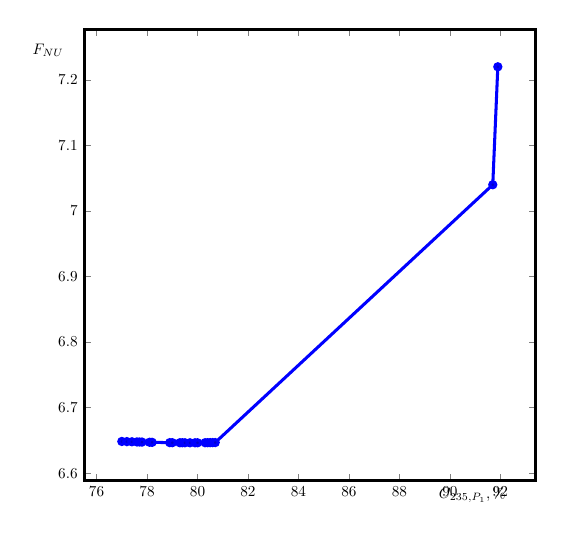
\begin{tikzpicture}[,
scale=0.55]
\begin{axis}[
  xlabel style = {{at={(axis description cs:.86,0)}}},
  ylabel = {$F_{NU}$},
  ylabel style = {{at={(axis description cs:-0.08,.925)},rotate=270,anchor=south}},
  xlabel = {$C_{235,P_1}, \%$},
  width=12cm, height=12cm, line width=2pt
]

\addplot+ coordinates {
  (77.0, 6.648369301601674)
  (77.2, 6.6481081422427755)
  (77.4, 6.6478609680670795)
  (77.60000000000001, 6.647628620667707)
  (77.7, 6.647518634806713)
  (77.8, 6.647412135764082)
  (78.10000000000001, 6.647118512130983)
  (78.2, 6.64702925961305)
  (78.9, 6.6465428786148735)
  (79.0, 6.646493966987278)
  (79.3, 6.646383406485429)
  (79.4, 6.646358460860561)
  (79.5, 6.646339791250357)
  (79.7, 6.646321811441468)
  (79.9, 6.646330897249658)
  (80.0, 6.646346113745254)
  (80.30000000000001, 6.64643598238657)
  (80.4, 6.646481376154359)
  (80.5, 6.646534553797508)
  (80.60000000000001, 6.646596419821)
  (80.7, 6.646666619197229)
  (91.7, 7.040023902346512)
  (91.9, 7.219931649864452)
};

\end{axis}
\end{tikzpicture}


% \caption{{Зависимость удельного расхода природного урана от концентрации $^{235}$U в потоке легкой фракции первого каскада от концентрации $^{235}$U в потоке легкой фракции первого каскада{\label{Fnu}}}}
% \end{minipage}
% \end{figure}


% \begin{figure}
%     \centering
%     \begin{minipage}{.5\textwidth}
%       \centering
%       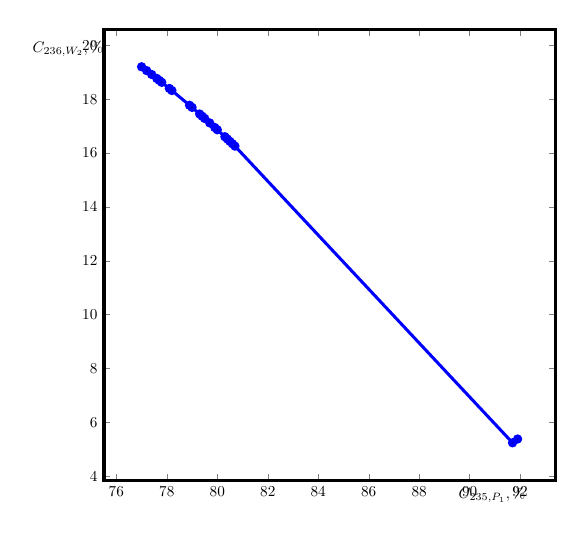
\begin{tikzpicture}[,
scale=0.55]
\begin{axis}[
  xlabel style = {{at={(axis description cs:.86,0)}}},
  ylabel = {$C_{236,W_2}, \%$},
  ylabel style = {{at={(axis description cs:-0.08,.925)},rotate=270,anchor=south}},
  xlabel = {$C_{235,P_1}, \%$},
  width=12cm, height=12cm, line width=2pt
]

\addplot+ coordinates {
  (77.0, 19.20354995742973)
  (77.2, 19.062157204472125)
  (77.4, 18.918608578311712)
  (77.60000000000001, 18.77292307609964)
  (77.7, 18.69928324668024)
  (77.8, 18.62511484136794)
  (78.10000000000001, 18.39945499658532)
  (78.2, 18.323189450313432)
  (78.9, 17.7750211540419)
  (79.0, 17.69470419345584)
  (79.3, 17.450804234311285)
  (79.4, 17.368538182322084)
  (79.5, 17.28579302654852)
  (79.7, 17.118891391179204)
  (79.9, 16.95013137456677)
  (80.0, 16.865062761747023)
  (80.30000000000001, 16.607172887205294)
  (80.4, 16.52032848882317)
  (80.5, 16.433051693388173)
  (80.60000000000001, 16.345346694722917)
  (80.7, 16.257219150399703)
  (91.7, 5.237747790489424)
  (91.9, 5.378427324120691)
};

\end{axis}
\end{tikzpicture}


% \caption{{Зависимость  концентрации $^{236}$U в потоке тяжелой фракции второго каскада $W_2$ от концентрации $^{235}$U в потоке легкой фракции первого каскада{\label{SW_l}}}}
%     \end{minipage}%
%     \begin{minipage}{.5\textwidth}
%       \centering
%       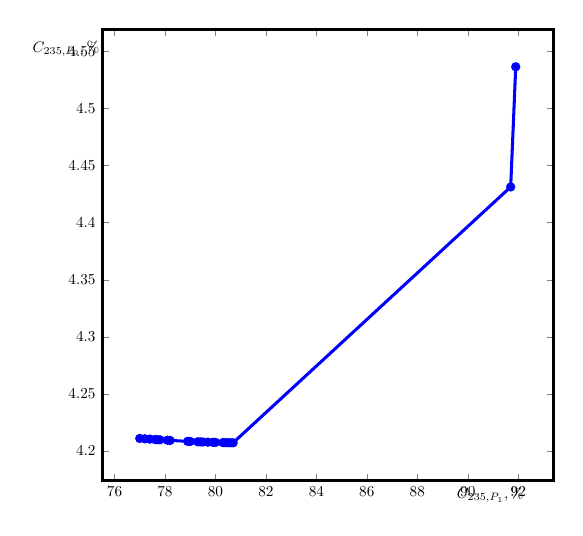
\begin{tikzpicture}[,
scale=0.55]
\begin{axis}[
  xlabel style = {{at={(axis description cs:.86,0)}}},
  ylabel = {$C_{235,P_0}, \%$},
  ylabel style = {{at={(axis description cs:-0.08,.925)},rotate=270,anchor=south}},
  xlabel = {$C_{235,P_1}, \%$},
  width=12cm, height=12cm, line width=2pt
]

\addplot+ coordinates {
  (77.0, 4.21096972553198)
  (77.2, 4.210659839435366)
  (77.4, 4.210358740398204)
  (77.60000000000001, 4.21006690040276)
  (77.7, 4.209924833527194)
  (77.8, 4.2097849356492505)
  (78.10000000000001, 4.209381303630404)
  (78.2, 4.209252109719451)
  (78.9, 4.208432990894553)
  (79.0, 4.208328602741027)
  (79.3, 4.208037634529696)
  (79.4, 4.207947919570074)
  (79.5, 4.207862044083126)
  (79.7, 4.207702088087786)
  (79.9, 4.207558613523564)
  (80.0, 4.207493381041667)
  (80.30000000000001, 4.207324521438157)
  (80.4, 4.207277603916635)
  (80.5, 4.2072354018766385)
  (80.60000000000001, 4.207198471785372)
  (80.7, 4.207166582032032)
  (91.7, 4.431200154395044)
  (91.9, 4.53639624850586)
};

\end{axis}
\end{tikzpicture}


% \caption{{Зависимость концентрации $^{235}$U в НОУ-разбавителе от концентрации $^{235}$U в потоке легкой фракции первого каскада{\label{Fnu}}}}
% \end{minipage}
% \end{figure}